% (The MIT License)
%
% Copyright (c) 2023-2024 Yegor Bugayenko
%
% Permission is hereby granted, free of charge, to any person obtaining a copy
% of this software and associated documentation files (the 'Software'), to deal
% in the Software without restriction, including without limitation the rights
% to use, copy, modify, merge, publish, distribute, sublicense, and/or sell
% copies of the Software, and to permit persons to whom the Software is
% furnished to do so, subject to the following conditions:
%
% The above copyright notice and this permission notice shall be included in all
% copies or substantial portions of the Software.
%
% THE SOFTWARE IS PROVIDED 'AS IS', WITHOUT WARRANTY OF ANY KIND, EXPRESS OR
% IMPLIED, INCLUDING BUT NOT LIMITED TO THE WARRANTIES OF MERCHANTABILITY,
% FITNESS FOR A PARTICULAR PURPOSE AND NONINFRINGEMENT. IN NO EVENT SHALL THE
% AUTHORS OR COPYRIGHT HOLDERS BE LIABLE FOR ANY CLAIM, DAMAGES OR OTHER
% LIABILITY, WHETHER IN AN ACTION OF CONTRACT, TORT OR OTHERWISE, ARISING FROM,
% OUT OF OR IN CONNECTION WITH THE SOFTWARE OR THE USE OR OTHER DEALINGS IN THE
% SOFTWARE.

\documentclass{article}
\usepackage{../sqm}
\newcommand*\thetitle{Static Analysis}
\begin{document}

\plush{\sqmTitlePage{23}{}}

\qte
  [Steven Johnson]
  {steven-johnson.jpg}
  {\textbf{Lint} is a command which examines C source programs, detecting a number of \ul{bugs} and \ul{obscurities}. It enforces the type rules of C more strictly than the C compilers. It may also be used to enforce a number of \ul{portability restrictions} involved in moving programs between different machines and/or operating systems. Another option detects a number of \ul{wasteful}, or \ul{error prone}, constructions which nevertheless are, strictly speaking, legal.}
  {johnson1977lint}

% Extended static checking for Java

% https://dl.acm.org/doi/pdf/10.1145/1287624.1287633?casa_token=f0xMwXQyTGUAAAAA:9D4WEXeruGVgiyZrUvtOtIw75G4tZJCGDN9wxfRMzVyrsbQHep7Pdzh-QKtKs71zTl-jeGZaaeIXPpQ

\plush{\pptBanner{Why do JavaScript developers use linters?}
\begin{itemize}
  \setlength\itemsep{0em}
  \item Prevent Errors
  \item Augment Test Suites
  \item Avoid Ambiguous and Complex Code
  \item Maintain Code Consistency
  \item Faster Code Review
  \item Spare Developers' Feelings
  \item Save Discussion Time
  \item Learn About JavaScript
  \end{itemize}
  \source{tomasdottir2017and}}

\plush{\pptBanner{My Favorite Static Analyzers}
\begin{itemize}
    \item Java:
      \href{https://spotbugs.github.io/}{SpotBugs},
      \href{https://checkstyle.sourceforge.io/}{Checkstyle},
      \href{https://pmd.github.io/}{PMD},
      \href{https://www.qulice.com}{Qulice}\citep{bugayenko2014blog0813} for Java
    \item C++:
      \href{https://clang.llvm.org/extra/clang-tidy/}{Clang-Tidy}
    \item Rust:
      \href{https://github.com/rust-lang/rust-clippy}{clippy}
  \end{itemize}}

\qte
  [Krist{\'\i}n Fj{\'o}la T{\'o}masd{\'o}ttir]
  {kristin-tomasdottir.jpg}
  {Every single interview participant mentioned that one of the reasons why they use a linter is to maintain code \ul{consistency}.}
  {tomasdottir2018adoption}
\pitch{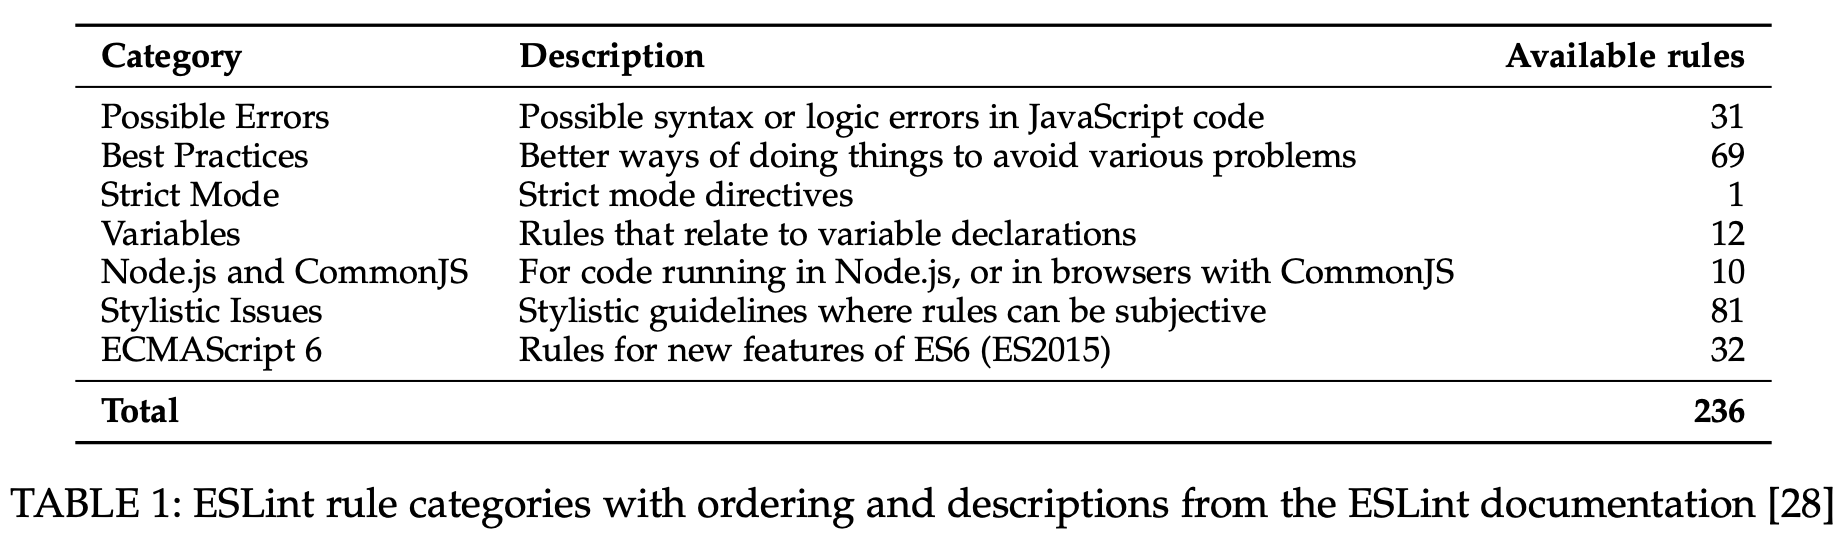
\includegraphics[width=.95\linewidth]{rules.png}
  \source{tomasdottir2018adoption}}

\qte
  [Florian Oberm{\"u}ller]
  {florian-obermuller.jpg}
  {We introduce the concept of \ul{code perfumes} as the counterpart to \ul{code smells}, indicating the correct application of programming practices considered to be good. Using a catalogue of 25 code perfumes for, we empirically demonstrate that these represent frequent practices in, and we find that better programs indeed contain more code perfumes.}
  {obermuller2021code}


\end{document}
